\documentclass[11pt]{report}
\usepackage{fullpage}
%\usepackage{sourcesanspro, sourcecodepro}
\usepackage{minted}
\usepackage{graphicx}
\usepackage{awesomebox}
\usepackage{hyperref}
\usepackage[a4paper, total={6in, 8in}, margin=0.75in]{geometry}
\usepackage{etoolbox}
\makeatletter
\patchcmd{\chapter}{\if@openright\cleardoublepage\else\clearpage\fi}{}{}{}
\RequirePackage[T1]{fontenc}
\RequirePackage[default,light,black]{roboto}

\hypersetup{
    colorlinks=true,
    linkcolor=blue,
    citecolor=blue,
    filecolor=blue,
    urlcolor=blue,
    pdfborder={0 0 0}
}

\graphicspath{{./images/}}

\title{APSC 258: Lab 6 Manual}
\author{Andre Cox  \\ Scott Halston}

\begin{document}
\maketitle
\tableofcontents

% page break
\clearpage

\chapter{Introduction}
\section{Introducing Droppout Layers}
In our last lab, you improved your self-driving neural networks by introducing convolution layers. Hopefully, by adding convolution layers, you were able to achieve a low training and testing mean squared error (MSE) value. Getting a low training MSE was probably much easier than achieving a low testing MSE value. This is because your model became overfit to the training data. Overfitting is when the model has learned the details and noise of the training data but has not learned the general shape of the data. To combat this, we will introduce dropout layers in this lab manual.

\section{Overfitting}
Overfitting occurs when a model is trained in a way that produces a model that fits exactly against its training data. When a model is overfitted, the model cannot predict unseen data accurately. Understanding this concept through words can be difficult; below are some graphs to help.

\begin{center}
    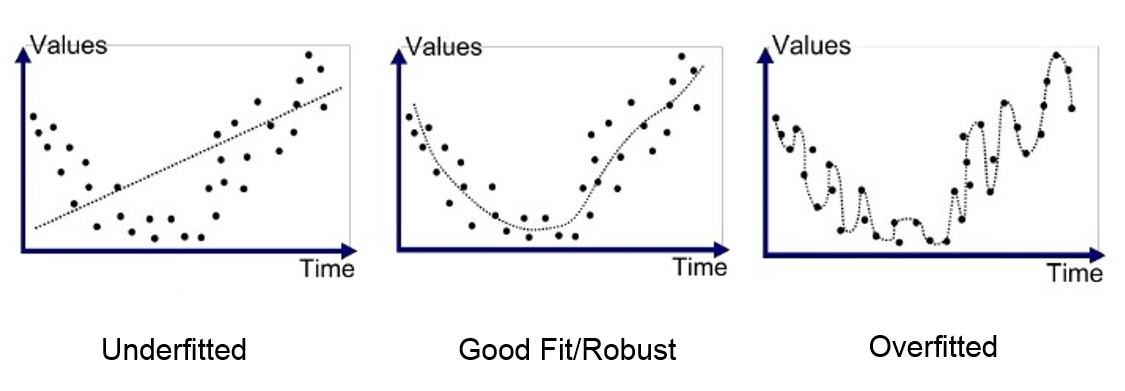
\includegraphics[scale=0.325]{./images/overfitexample.png}
\end{center}

\section{Dropout Layers}
We introduce dropout layers to combat overfitting our models. A dropout layer is a straightforward function that randomly drops training data to disrupt the model from becoming overfitted. An example of this can be seen below.

\begin{center}
    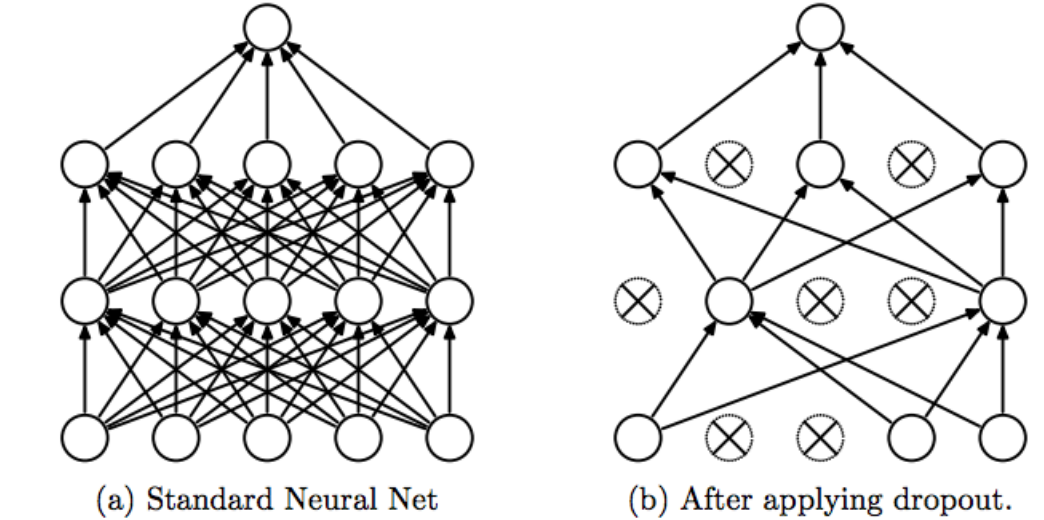
\includegraphics[scale=0.2]{./images/dropoutexample.png}
\end{center}



\chapter{Implementation}
Now that we better understand dropout layers, we can use them in our neural networks.

\section{Dropout Layers in Neural Networks}
Before we explain dropout layers, it is highly recommended that you first, go through the code below on your own to better your understanding of dropout layers.

\begin{minted}[linenos, fontfamily=courier, style=monokai, bgcolor=black, breaklines]{python}
    # First we'll import the layers we'll be using
    from keras.layers import Dense, Dropout # here's the dropout layer
    from keras.models import Sequential # here's the model we'll be using

    # Create the model
    model = Sequential()

    # now lets add some layers to the model
    model.add(Dense(units=1, activation='relu')) # first layer
    model.add(Dense(units=25, activation='relu')) # second layer
    model.add(Dropout(0.2)) # dropout layer with 20% of the units being set to zero
    model.add(Dense(units=25, activation='relu')) # third layer
    model.add(Dense(units=1, activation='sigmoid')) # output layer
\end{minted}

\section{Explanation}
In the sample code above, we can see that our model has four dense layers. In the center of the model, we have a dropout layer. This layer randomly sets 20 percent of the weights to zero. This is done to prevent the model from overfitting. 

\notebox{\textbf{Note:} We define percentages as floats between 0 and 1. This means, 0.2 would be 20 percent. You can experiment with different percentages in the dropout layer to see how the model performs.}


\chapter{Your Turn}
\section{Applying the Convolution Layer}
Now that you have a good grasp of dropout layers, we can apply it to our own neural networks. Open the model that you've been working on over the past 2 labs and try experimenting by adding dropout layer(s). See if multiple dropout layers function better than a single one and test what values of the dropout layer(s) provide the best results. Keep in mind that the location of your dropout layers will also have an impact.
Your goal in this lab is to try to decrease the loss of validation data. You can go about this in the following steps:

\begin{enumerate}
    \item{Take your model from the previous lab.}
    \item{Record your current loss on the training and validation data.}
    \item{Add a dropout layer to your model.}
    \item{Add a random dropout percentage. Somewhere between 0 and 1.}
    \item{Retrain your model.}
    \item{Record your current loss on the training and validation data.}
    \item{Repeat the process until you can't get the loss to decrease any more.}
\end{enumerate}

\tipbox{\textbf{Hint:} A good starting point for picking a random dropout percentage is 0.2 - 0.5. Most convolutional neural networks put the dropout layers in the Dense layers.}

\pagebreak

\chapter{Finishing Up}

Once you have implemented dropout layers in your model and are happy with the results, you can save your model. Once this is done have a go downloading it and running it on the PiCarV. If you need a reminder on how to do this, please refer to Lab 4.

\section{Finished!}
You now have all of the tools of neural networks available to you to make your model the best it can be! Your next lab manual will detail how your models will be graded and what you should be trying to achieve.

\end{document}
